\documentclass[12pt]{exam-zh}
\usepackage{array}
\usepackage{tabularx} % 用于自动调整列宽

\examsetup{
  page = {
    size            = a3paper,
    show-columnline = false
  },
  paren/show-paren = true,
  paren = {type = none},
    fillin/type = paren,
  style/fullwidth-stop = false, % 全宽的句号
  sealline = {
    show        = true,
    type       = everypage,
    circle-show = false,
    line-type   = dashed,
    line-xshift = 2mm,
    odd-info-content = {
    },
    odd-info-xshift = 12mm,
    text = {},
  },
  square = {
    x-length = 1.8em,
    y-length = 1.6em
  }
}

% 行内公式统一按照行间的样式
\everymath{\displaystyle}



\begin{document}

% 插入表格

% \begin{table}[h!]
% \begin{tabular}{|l|}
% \hline
% 学 \quad 校 \\ \hline
%     \\ \hline
% 班 \quad 级 \\ \hline
%     \\ \hline
% 姓 \quad 名 \\ \hline
%     \\ \hline
% 考 \quad 号 \\ \hline
%     \\ \hline
% \end{tabular}
% \end{table}

\chapter{2024-2025第二学年度二年级数学期末测试卷}

% 得分情况
% \newcolumntype{C}{>{\centering\arraybackslash}m{1.5cm}}
% \begin{table}[htbp]
%     \centering
%     \begin{tabular*}{\columnwidth}{@{\extracolsep{\fill}}|C|C|C|C|C|C|C|C|}
%         \hline
%         题号 & 一 & 二 & 三 & 四 & 五 & 六 & 总分 \\ \hline
%         得分 &   &   &   &   &   &   &    \\ \hline
%     \end{tabular*}
% \end{table}



\newcolumntype{C}{>{\centering\arraybackslash}m{1.5cm}} % 定义居中对齐的列类型
\begin{table}[htbp]
    \centering
    \begin{tabular}{|C|C|C|C|C|C|C|} % 6列,对应一、二、三、四、五、总分
        \hline
        题号 & 一 & 二 & 三 & 四 & 五 & 总分 \\ \hline
        得分 &   &   &   &   &   &   \\ \hline
    \end{tabular}
\end{table}
% 得分情况
% \newcolumntype{C}{>{\centering\arraybackslash}m{1.5cm}}
% \begin{table}[htbp]
%     \centering
%     \begin{tabular*}{\columnwidth}{@{\extracolsep{\fill}}|C|C|C|C|C|C|C|C|}
%         \hline
%         题号 & 一 & 二 & 三 & 四 & 五 & 六 & 总分 \\ \hline
%         得分 &   &   &   &   &   &   &    \\ \hline
%     \end{tabular*}
% \end{table}


% 第一大题
\section{
  填一填、我能行。
  (每空1分,共40分)
}

% 设置填空的样式以及不显示三角形
\examsetup{fillin/no-answer-type=none}

% 1.
\begin{question}
画一画、填一填。
\begin{multifigures}
\item[读作:\fillin[width=10em][]] 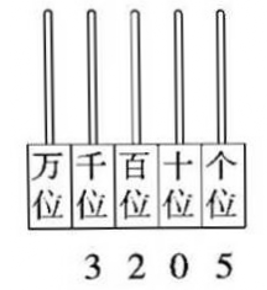
\includegraphics [height =3cm]{1.png}
\item[读作:\fillin[width=10em][]] 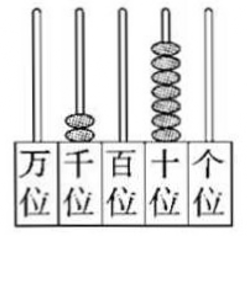
\includegraphics [height =3cm]{2.png}
\item[读作:\fillin[width=10em][]] 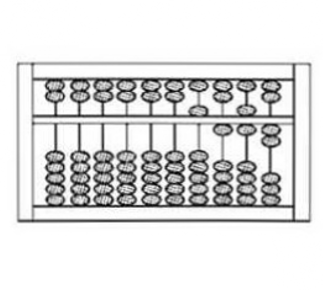
\includegraphics [height =3cm]{3.png}
\end{multifigures}
\end{question}

% 2.
\begin{question}
29个十是\fillin[width=3em][],1800里面有\fillin[width=3em][]个百。10个一千是\fillin[width=3em][]。
\end{question}

% 3.
\begin{question}
36里面有\fillin[width=3em][]个9。被除数是42,除数是7,商是\fillin[width=3em][]。
\end{question}

4.
\begin{question}
24÷4=6,表示把\fillin[width=3em][]平均分成\fillin[width=3em][]份,每份是\fillin[width=3em][]。还表示24里面有\fillin[width=3em][]个\fillin[width=3em][]。
\end{question}

% 5.
\begin{question}
在$\textbigcircle$里填上“>”、“<”或“=”。

% 插入空格
2800克 $\textbigcircle$ 3千克 $\quad\quad$ 980克 $\textbigcircle$ 1千克 $\quad\quad$ 899 $\textbigcircle$ 1001 $\quad\quad$ 3420 $\textbigcircle$ 3240

% 插入空格
3000+2000 $\textbigcircle$ 5600 $\quad\quad$ 32 $\div$ 8 $\textbigcircle$ 12 $\div$ 3 $\quad\quad$ 52+18 $\textbigcircle$ 52 $-$ 18
\end{question}

% 6.
\begin{question}
一只鸡重1988\fillin[width=3em][],约是2\fillin[width=3em][]。一台冰箱的售价是3998元,一个电磁炉的售价是1058元,买一台冰箱比买一个电磁炉大约贵\fillin[width=3em][]元。
\end{question}

% 7.
\begin{question}
与1999相邻的两个数是\fillin[width=3em][]和\fillin[width=3em][]。
\end{question}

% 8.
\begin{question}
3007是\fillin[width=3em][]位数。这个数读作\fillin[width=10em][]。这个数中的“3”在\fillin[width=3em][]位上,表示\fillin[width=10em][];7在\fillin[width=3em][]位上,表示\fillin[width=10em][]。
\end{question}

% 9.
\begin{question}
用6、4、1、0组成的最大的四位数是\fillin[width=3em][],组成的最小的四位数是\fillin[width=3em][]。
\end{question}

% 10.
\begin{question}
    \raisebox{0.7ex}{
    % 方框1
    
\begin{tikzpicture}[baseline=(current bounding box.center)]
        \pgfmathsetlengthmacro{\radius}{0.5\baselineskip}
        \draw[line width=1pt] (0,0) rectangle (\radius,\radius); % 指定具体数值(1pt)
        \draw[thick] (0,0) rectangle (\radius,\radius); % 0.8pt(默认thick值)
    \end{tikzpicture}
    % 方框2
    
\begin{tikzpicture}[baseline=(current bounding box.center)]
        \pgfmathsetlengthmacro{\radius}{0.5\baselineskip}
        \draw[line width=1pt] (0,0) rectangle (\radius,\radius); % 指定具体数值(1pt)
        \draw[thick] (0,0) rectangle (\radius,\radius); % 0.8pt(默认thick值)
    \end{tikzpicture} 
    % 圆1
    
\begin{tikzpicture}[baseline=(current bounding box.center)]
        % 计算半径:行高的一半
        \pgfmathsetlengthmacro{\radius}{0.5\baselineskip}
        % 绘制同心圆
        \draw[line width=1pt] (0,0) circle (0.5*\radius);      % 外圆(直径=行高)
        % \draw[line width=1pt] (0,0) circle (0.5*0.5*\radius);  % 内圆(半径为外圆一半)
    \end{tikzpicture}
    % 圆2
    
\begin{tikzpicture}[baseline=(current bounding box.center)]
        % 计算半径:行高的一半
        \pgfmathsetlengthmacro{\radius}{0.5\baselineskip}
        % 绘制同心圆
        \draw[line width=1pt] (0,0) circle (0.5*\radius);      % 外圆(直径=行高)
        \draw[line width=1pt] (0,0) circle (0.5*0.5*\radius);  % 内圆(半径为外圆一半)
    \end{tikzpicture}
    % 方框1
    
\begin{tikzpicture}[baseline=(current bounding box.center)]
        \pgfmathsetlengthmacro{\radius}{0.5\baselineskip}
        \draw[line width=1pt] (0,0) rectangle (\radius,\radius); % 指定具体数值(1pt)
        \draw[thick] (0,0) rectangle (\radius,\radius); % 0.8pt(默认thick值)
    \end{tikzpicture}
    % 方框2
    
\begin{tikzpicture}[baseline=(current bounding box.center)]
        \pgfmathsetlengthmacro{\radius}{0.5\baselineskip}
        \draw[line width=1pt] (0,0) rectangle (\radius,\radius); % 指定具体数值(1pt)
        \draw[thick] (0,0) rectangle (\radius,\radius); % 0.8pt(默认thick值)
    \end{tikzpicture} 
    % 圆1
    
\begin{tikzpicture}[baseline=(current bounding box.center)]
        % 计算半径:行高的一半
        \pgfmathsetlengthmacro{\radius}{0.5\baselineskip}
        % 绘制同心圆
        \draw[line width=1pt] (0,0) circle (0.5*\radius);      % 外圆(直径=行高)
        % \draw[line width=1pt] (0,0) circle (0.5*0.5*\radius);  % 内圆(半径为外圆一半)
    \end{tikzpicture}
    % 圆2
    
\begin{tikzpicture}[baseline=(current bounding box.center)]
        % 计算半径:行高的一半
        \pgfmathsetlengthmacro{\radius}{0.5\baselineskip}
        % 绘制同心圆
        \draw[line width=1pt] (0,0) circle (0.5*\radius);      % 外圆(直径=行高)
        \draw[line width=1pt] (0,0) circle (0.5*0.5*\radius);  % 内圆(半径为外圆一半)
    \end{tikzpicture}}
 $\dots$按这样的规律排列,第19个图形是\fillin[width=3em][],第28个图形是\fillin[width=3em][]。
\end{question}

% 11.
\begin{question}
    \raisebox{0.7ex}{
    
\begin{tikzpicture}[baseline=(current bounding box.center)]
        \pgfmathsetlengthmacro{\radius}{0.5\baselineskip}
        \draw[line width=1pt] (0,0) rectangle (\radius,\radius); % 指定具体数值(1pt)
        \draw[thick] (0,0) rectangle (\radius,\radius); % 0.8pt(默认thick值)
    \end{tikzpicture}}
    $\div$
    \hspace{-0.9em}
    \raisebox{0.7ex}{
    
\begin{tikzpicture}[baseline=(current bounding box.center)]
        % 计算半径:行高的一半
        \pgfmathsetlengthmacro{\radius}{0.5\baselineskip}
        % 绘制同心圆
        \draw[line width=1pt] (0,0) circle (0.5*\radius);      % 外圆(直径=行高)
        % \draw[line width=1pt] (0,0) circle (0.5*0.5*\radius);  % 内圆(半径为外圆一半)
    \end{tikzpicture}}
    =6$\dots \dots $4 ,
    \raisebox{0.7ex}{
    
\begin{tikzpicture}[baseline=(current bounding box.center)]
        % 计算半径:行高的一半
        \pgfmathsetlengthmacro{\radius}{0.5\baselineskip}
        % 绘制同心圆
        \draw[line width=1pt] (0,0) circle (0.5*\radius);      % 外圆(直径=行高)
        % \draw[line width=1pt] (0,0) circle (0.5*0.5*\radius);  % 内圆(半径为外圆一半)
    \end{tikzpicture}}
    最小填
    \fillin[width=3em][],这时
    \raisebox{0.7ex}{
    
\begin{tikzpicture}[baseline=(current bounding box.center)]
        \pgfmathsetlengthmacro{\radius}{0.5\baselineskip}
        \draw[line width=1pt] (0,0) rectangle (\radius,\radius); % 指定具体数值(1pt)
        \draw[thick] (0,0) rectangle (\radius,\radius); % 0.8pt(默认thick值)
    \end{tikzpicture}}
    =\fillin[width=3em][]。
\end{question}
% -----------------------------


\examsetup{
    question/show-answer = false,    
    fillin/type=paren,
    paren/show-paren = true,
    paren = {type = hfill},
}

% 第二大题
\section{
  辨一辨、我最棒。
  (每题1分,共5分)
}

% 1.
\begin{question}[index=1]
把18个苹果分给6个小朋友,每个小朋友分到的一定是3个苹果。  \paren[ ]
\end{question}

% 2.
\begin{question}[index=2]
1000克的棉花比1千克的铁重。                                \paren[ ]
\end{question}
% 3.
\begin{question}[index=3]
$13-8=5$和$5\times8=40$这两个算式合并成一个综合算式是$13-8\times5=40$。 \paren[ ]
\end{question}
% 4.
\begin{question}[index=4]
1002前边的第3个数是999,后边的第3个数是1004。        \paren[ ]
\end{question}
% 5.
\begin{question}[index=5]
50克和50厘米,属于不同的计量单位,不能比较大小。       \paren[ ]
\end{question}


% +  - \times {\div} 

% 第三大题
\section{
  选一选(每空1分,共6分)
}

% 1.
\begin{question}[index=1]
8
\hspace{-0.5em}\raisebox{0.7ex}{
    
\begin{tikzpicture}[baseline=(current bounding box.center)]
        \pgfmathsetlengthmacro{\radius}{0.5\baselineskip}
        \draw[line width=1pt] (0,0) rectangle (\radius,\radius);
    \end{tikzpicture}}
    \hspace{-0.25em}6 $<$861,
    \raisebox{0.7ex}{
    
\begin{tikzpicture}[baseline=(current bounding box.center)]
        \pgfmathsetlengthmacro{\radius}{0.5\baselineskip}
        \draw[line width=1pt] (0,0) rectangle (\radius,\radius); % 指定具体数值(1pt)
        \draw[thick] (0,0) rectangle (\radius,\radius); % 0.8pt(默认thick值)
    \end{tikzpicture}}
    里可以填\fillin[width=3em][]个适当的数字。
\begin{choices}
\item 5
\item 6
\item 7
\end{choices}
\end{question}

% 2.
\begin{question}[index=2]
下面三位同学每人拿一种水果,分别是桃、香蕉、和梨。小强说:“我拿的是桃。”小芳说:“我拿的不是梨。”小丽拿的是\fillin[width=3em][]小芳拿的是\fillin[width=3em][]。
\begin{choices}
\item 桃
\item 香蕉
\item 梨
\end{choices}
\end{question}

% 3.
\begin{question}[index=3]
已经包了24个粽子,至少再包\fillin[width=3em][]个粽子,能正好平均分给9个小朋友。
\begin{choices}
\item 2
\item 3
\item 4
\end{choices}
\end{question}

% 4.
\begin{question}[index=4]
下列标志中,是轴对称的有\fillin[width=3em][]个。
\begin{multifigures}[columns=5,xshift=10mm]
    \item 
\includegraphics[height=2cm]{4.png}
    \item 
\includegraphics[height=2cm]{5.png}
    \item 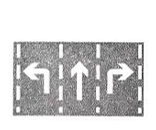
\includegraphics[height=2cm]{6.png}
    \item 
\includegraphics[height=2cm]{7.png}
    \item 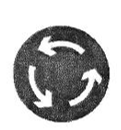
\includegraphics[height=2cm]{8.png}
\end{multifigures}
\begin{choices}
\item 1
\item 2
\item 3
\item 4
\end{choices}
\end{question}

% 5.
\begin{question}[index=5]
下列现象中,\fillin[width=3em][]不属于平移。
\begin{choices}
\item 风车迎风转动
\item 国旗沿着旗杆升起
\item 电梯的升降
\item 箱子在水平地面上沿直线移动
\end{choices}
\end{question}

% 第四大题
\section{
  算一算(共21分)
}

% 1.
\begin{question}[index=1]
直接写得数。(5分)
\hspace{-11.5em}% 负值左移(单位:em或cm)
\raisebox{-7ex}{
\begin{calculations}[index=1,label={},columns=5,hsep=0.5cm,vsep=0.2cm]
\item 19 $\div$ 2 = 
\item 48 $\div$ 8 = 
\item 500 + 1000 = 
\item 2600 $-$ 1000 = 
\item 3300 + 400 = 
\item 30 $\div$ 7 = 
\item 6 $\div$ 6 = 
\item 8000 $-$ 2000 = 
\item 1500 $-$ 900 = 
\item 4200 + 3000 = 
\end{calculations}}
\end{question}

% 2.
\begin{question}[index=2]
脱式计算。(每题2分,共8分)
\hspace{-15em}% 负值左移(单位:em或cm)
\raisebox{-4ex}{
\begin{calculations}[index=2,label={},columns=4,hsep=1.5cm,vsep=0cm]
\item 35 + 21 $\div$ 7
\item 8 $\times$ 3 $\div$ 4
\item 4 $\times$ (72 $\div$ 9)
\item 42 $\div$ (90 $-$ 83)
\end{calculations}}
\end{question}

\vspace{2.5cm} % 添加1厘米垂直空白

% 3.
\begin{question}[index=3]
竖式计算。(每题2分,共8分)
\hspace{-15em}% 负值左移(单位:em或cm)
\raisebox{-4ex}{
\begin{calculations}[index=3,label={},columns=4,hsep=2cm,vsep=0cm]
\item 32 $\div$ 8 =
\item 50 $\div$ 6 =
\item 49 $\div$ 9 =
\item 66 $\div$ 7 =
\end{calculations}}
\end{question}

\vspace{2.5cm} % 添加1厘米垂直空白

% 第五大题
\section{
  解决问题。(共28分)
}

% 1.
\begin{problem}[index=1]
赵叔叔家要挖总长60米的水沟,已经挖了15米。剩下的用5天挖完,平均每天要挖多少米?(4分)
\end{problem}

\vspace{3cm} % 添加1厘米垂直空白

% 2.
\begin{problem}[index=2]
一支钢笔9元,一支铅笔6元,买4支钢笔的钱可以买几支铅笔?(4分)
\end{problem}

\vspace{3cm} % 添加1厘米垂直空白

% 3.
\begin{problem}[index=3]
王叔叔要做50个灯笼,他每天最多可以做8个。至少需要多少天才能做完?(4分)
\end{problem}
\vspace{3cm} % 添加1厘米垂直空白
% 4.
\begin{problem}[index=4]
植树
\begin{multifigures}[columns=3,xshift=15mm]
\item 
\includegraphics[height=2.5cm]{9.png}
\item 
\includegraphics[height=2.5cm]{10.png}
\item 
\includegraphics[height=2.5cm]{11.png}
\end{multifigures}

(1)柳树比杨树多植了多少棵?(3分)

\vspace{3cm} % 添加1厘米垂直空白

(2)松树和杨树一共植了多少棵?(3分)

\vspace{2.5cm} % 添加1厘米垂直空白

\end{problem}

% 5.
\begin{problem}[index=5]
    有一条500厘米长的彩带,包扎三盒礼物已经用掉了300厘米,还需要240厘米做蝴蝶结。剩下的彩带够吗?(4分)
\end{problem}
\vspace{2.5cm} % 添加1厘米垂直空白

% 6.
\begin{problem}[index=6]
红红调查的本班同学最喜欢吃的水果情况如下:(每格0.5分,共2分)

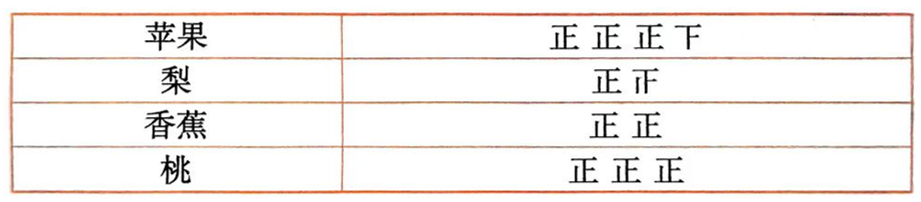
\includegraphics[scale=0.4]{12.png}

(1)把调查的结果填入下表中。

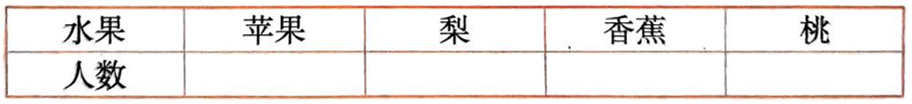
\includegraphics[scale=0.4]{13.png}

(2)最喜欢吃\fillin[width=3em][]的人数最多,最喜欢吃\fillin[width=3em][]的人数最少。(2分)

(3)如果本班同学去郊游,那么应该多买哪种水果?为什么?(2分)
\end{problem}


\end{document}
